\documentclass[10pt,a4paper]{report}
\usepackage[utf8]{inputenc}
\usepackage{amsmath}
\usepackage{amsfonts}
\usepackage{amssymb}
\usepackage{graphicx}
\begin{document}
\begin{LARGE}
\textbf{MSMExplorer Walkthrough}
\end{LARGE}
\section*{Introduction}

Welcome to MSMExplorer! This document is intended as a guided walkthrough of  most of MSMExplorer's features. For a thorough reference, please see the file \texttt{REFERENCE\_TUTORIAL.pdf}. Additionally, new users are encouraged to visit   \texttt{https://simtk.org/docman/?group\_id=529} where links to walkthrough videos may be found. Please note that this walkthrough is intended as relatively comprehensive, and that mastery of all the steps presented here is not required for usage of MSMExplorer. Understanding through step 3 should provide basic facility with the program and through step 6 intermediate facility.

\subsection*{0. Starting MSMExplorer}
MSMExplorer requires Java 1.6. There are two ways to start MSMExplorer. 

\subparagraph{1. From the Command Line}
From the command line on a unix-based machine, navigate to the base MSMExplorer directory and execute \texttt{./run.sh} (note that this command must be executed from the MSMExplorer base directory).

\subparagraph*{2. From the File Browser}
In a GUI file browser, open the folder ``dist'' in the MSMExplorer main directory. Double click on MSMExplorer.jar to start MSMExplorer. 

\begin{figure}[h]
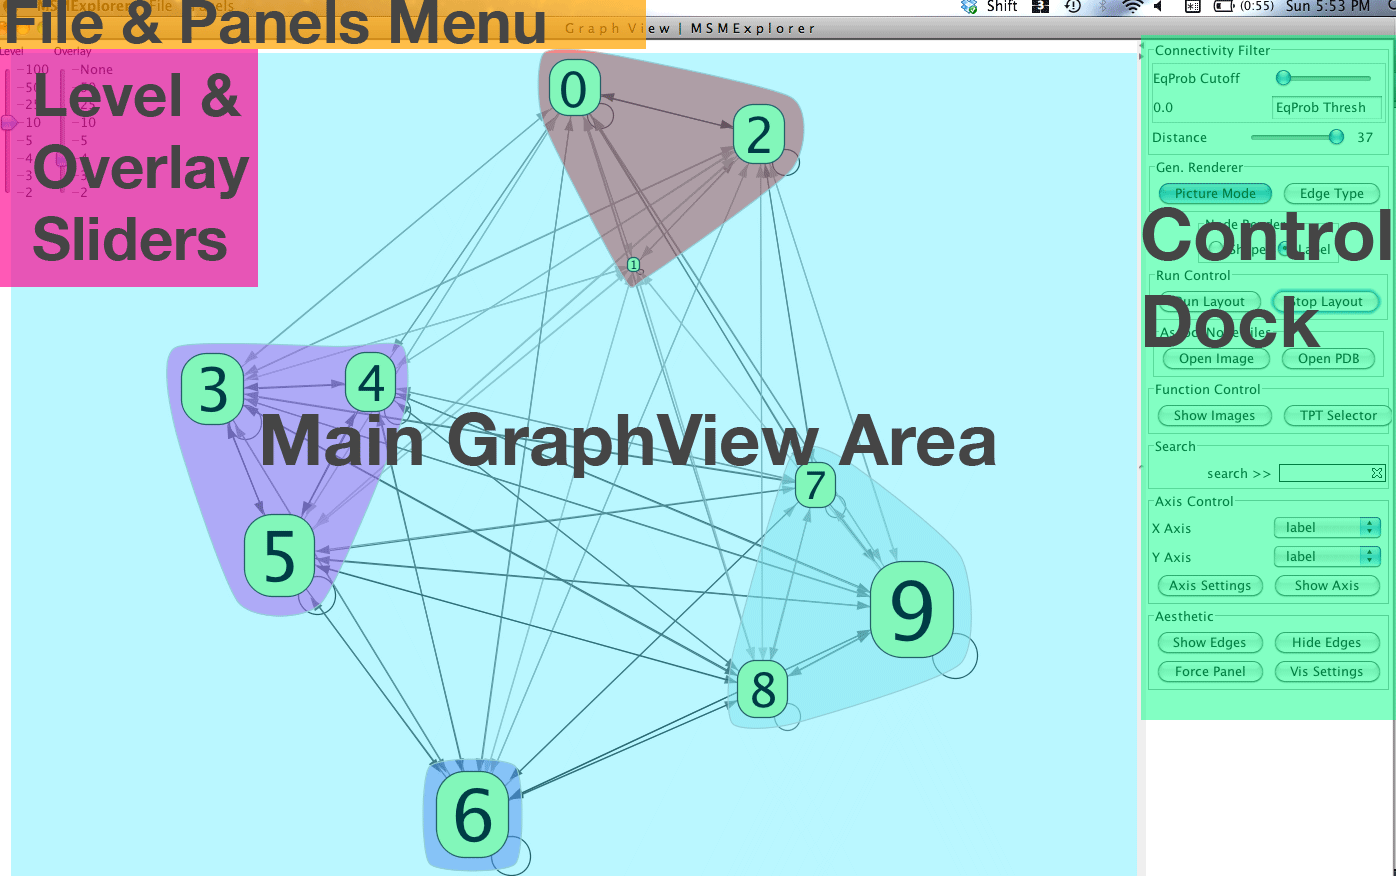
\includegraphics[scale=.25]{overview.png}
\caption{Location of basic controls areas referenced in this walkthrough}
\end{figure}


\section*{Visualizing MSMs}
When MSMExplorer is first started, select the "Graph View" option. A window will open with a simple toy 5 state model. Each node represents a set of conformations, and edges represent transitions between these sets of conformations. By default, edge shading indicates the probability of a transition along that edge, and node size indicates equilibrium probability of the corresponding macrostate. Click and drag a node to reposition it, click and drag on the background to pan, use the mouse wheel to zoom, and right click on the background to put the entire graph in the center of the screen.
\subsection*{1. Open an MSMs}
Let's load a more interesting MSM into MSMExplorer. Go to \emph{File $\rightarrow$ Open File} and navigate to the folder \emph{demos/tutorial} in the base MSMExplorer directory. Select \emph{tProb.mtx}. MSMExplorer will prompt you whether you want to use the file \emph{Populations.dat} it found automatically; in this case, we know this file contains the equilibrium probabilities for our model, so select \emph{Yes}. A new graph will appear in GraphView containing 25 nodes. This is a 25 state macrostate model of a folding simulation for Alanine Dipeptide.

\subparagraph*{Supported Filetypes}
MSMExplorer supports the filetypes output by MSMBuilder by default. For matricies, these are simple space delimited ASCII files for dense matricies (.dat or .txt) and MatrixMarket Coordinate General format for sparse matricies (.mtx). MSMExplorer additionally supports GraphML files (.graphml or .xml). Supplemental data columns (including equilibrium probabilities) should be provided in simple newline-delimited format. If your MSMs are produced with EMMA, there is a very simple script provided in the folder \emph{aux} that will convert EMMA matrix files into MSMBuilder formats.

\subsection*{2. Freeze layout}
The movement of the graph is a feature of MSMExplorer's layout algorithm. MSMExplorer uses a Force-Directed Layout algorithm -- where nodes are simulated as masses and edges as springs -- to automatically produce a useful layout for the graph. However, during analysis, we often prefer more direct control over the placement of nodes. To stop the layout at any time, select \emph{Stop Layout} on the panel at right (the \emph{Control Dock}). You may drag nodes to reposition them to more clearly reveal relevant structure.

\subsection*{3. Export a view}
Make sure the entire graph is in the main window by right clicking on the background of the GraphView window. Now, save an image of the current view of the graph by going to \emph{File$\rightarrow$Save Image}. SVG is the default option; change this to jpeg, and scale up the image 2X using the slider on the left of the save dialog. 

\begin{figure}[h]
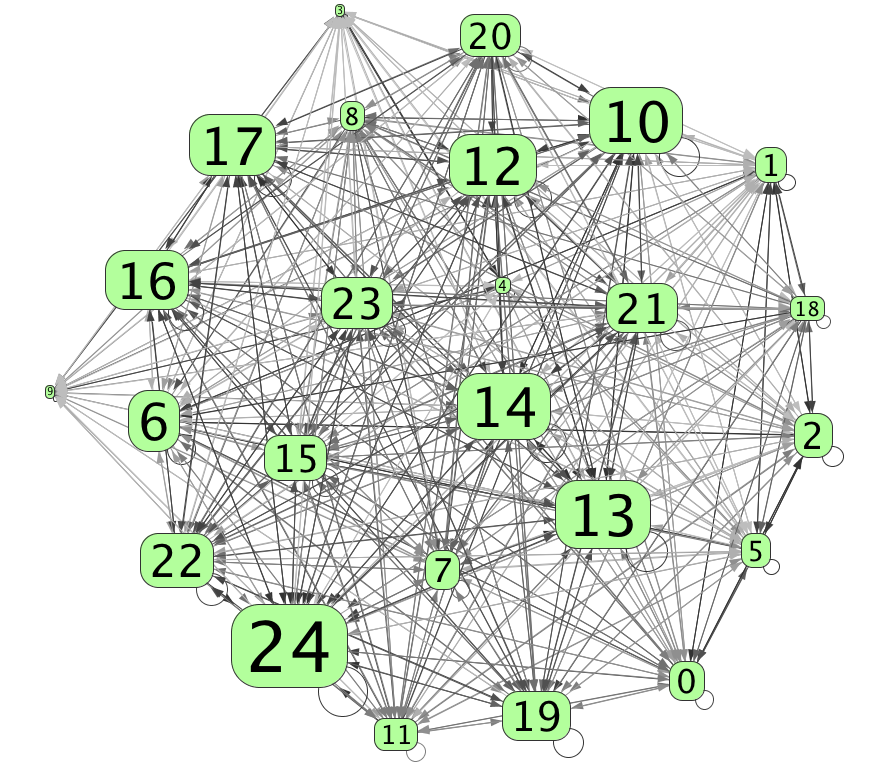
\includegraphics[scale=.3]{basic.png}
\caption{Default appearance of the 25 macrostate MSM}
\end{figure}

\subsection*{4. Import Data}
Now that we have an image of the basic data, let's import some additional data. Go to \emph{File $\rightarrow$ Add Data Column}. Name the column ``RMSD'', set the type to Double (default), and select graph.nodes for the visual group (also default), as we want to apply this new data to nodes. Select \emph{Load Data} and locate \emph{demos/tutorial/nodeDataCol.dat} in the MSMBuilder base directory. Note that you will need to change the filetype to \emph{.dat} to select the file. 
After loading the file, go to \emph{Panels $\rightarrow$ Node Panel}. A window depicting the backing node table with our new RMSD column should be present. 
Now, let's make use of our new data.

\subparagraph*{Custom Node Labels}
Node labels can be customized from the Node Panel; open the Node Panel again by navigating to \emph{Panels $\rightarrow$ Node Panel}. Double click on the entry in the ``label'' column for row ``0'' and enter ``Sink'' in its place; press enter to commit the change. Close the Node Panel and click on the main GraphView window. The label on the main graph should update accordingly. 

\subsection*{5. Axis Layout}
On the control panel, locate the \emph{Axis Control} panel. Change the \emph{X Axis} drop-down to eqProb to set the X-Axis to layout nodes by equilibrium probability, and set the Y-Axis to layout nodes by RMSD. Press \emph{Show Axis}. You now see a simple scatter plot of RMSD vs Equilibrium Probability. 

\subparagraph*{Prettifying the Scatter Plot}
To make all the points the same size, select \emph{Vis Settings}, and bring the two thumbs (squares with triangles on them) on the \emph{Node Size} slider together. Close the Vis Settings Panel. Remove the labels from the scatter plot points by selecting the \emph{Shape} radio button in the Node Renderer panel on the main Control Dock. Now hide edges by selecting \emph{Hide Edges} on the Control Dock. Add labels to the graph by selecting \emph{Axis Settings}; write``Equilibrium Probability'' in the X-axis box, and ``RMSD'' in the Y-axis box, and set the size of both to 32 point. Change the X and Y grid spacing to 100 to space out the gridlines more than default. Set the Grid Label size to 16. Select OK to confirm changes. Now toggle \emph{Show Axis} off and back on (press it twice) to refresh the Axis. You should now have the image below. Save this image as an SVG by going to \emph{File $\rightarrow$ Save Image}, selecting SVG as the filetype (selected by default) and saving as ``axis'' in your favorite directory.

\begin{figure}[h]
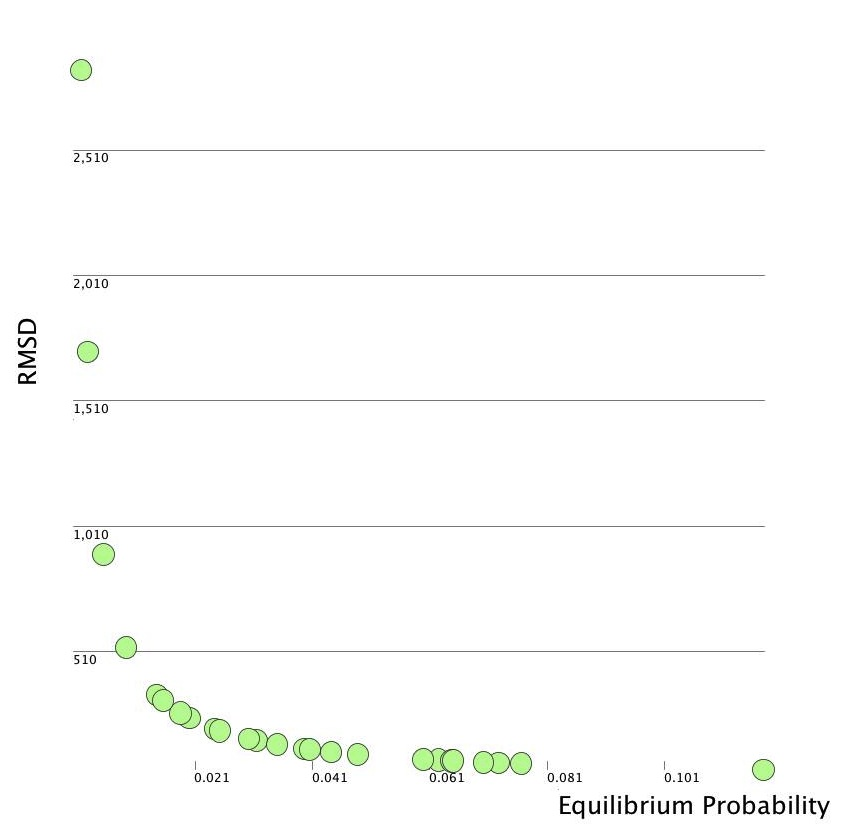
\includegraphics[scale=.3]{tut0.jpg}
\caption{Example of ``pretified'' scatter plot.}
\end{figure}

\subsection*{6. Linking Images and PDB Files}
In the \emph{demos/tutorial} folder resides a folder \emph{images} that contains 25 images in the proper filename format for MSMExplorer. Link these images with the current graph by going to \emph{File $\rightarrow$ Set Image Location} and select the folder \emph{demos/tutorial/images}. Now, find node 12 by searching for ``12'' in the search box on the Control Dock. Select this node by clicking on it, and select \emph{Open Image} on the Control Dock to bring up the associated image in another window. Close this window. Now click \emph{Show Images} on the Control Dock to show all images on top of nodes. 

\subparagraph*{Coercive Rendering}
If not all images are appearing properly or other half-baked rendering is observed, it could be that MSMExplorer is not actively refreshing its display, which tends to happen while layout is stopped. To fix this, click the background and pan around a little to wake the render queue up.

\subparagraph*{Layout Force Parameters}
The force parameters that are used to automatically lay out the graph in Graph View are adjustable. This is useful when nodes become large, either because the size threshold was adjusted in Vis Settings, or images were loaded, and overlap, hiding the connections between them. Open the force panel by selecting \emph{Force Panel} from the \emph{Panels} menu. Adjust the ``DefaultSpringLength'' parameter (the bottom in the panel) to about 800, and close the panel. Right click on the background of the GraphView window to zoom-to-fit and recenter the whole graph in the window. 

To link PDB files, click \emph{Open PDB} on the Control Dock with a node selected. Because you haven't already indicated the location of PDB files for this model, a dialog will pop up; navigate to and select \emph{demos/tutorial/PDBs}. The PDB for this node will automatically be opened via PyMol. Select a different node and select \emph{Open PDB} to open the PDB linked to the newly selected node.

Click \emph{Show Images} again to hide the images on nodes. 

\subsection*{7. Basic Visual Encoding Control and the Vis Settings Panel}
You can change what visual encodings -- such as color or size encodings -- represented in MSMExplorer via the Vis Settings panel, and the color and size ranges used. Open the panel by selecting \emph{Vis Settings} on the Control Dock. To adjust size range, pull on the thumbs on the \emph{Node Size} slider. Pull the right thumb up a bit to make the maximum size larger. Now, lets color nodes by RMSD; change the \emph{Node Color Field} to RMSD and change the End Color to a red by selecting \emph{End Color} and choosing, through whatever color chooser best suits your style, a nice red. Note that similar adjustments can be made for edge color and weight on the ``Edge'' tab of Vis Settings (and additional data can be imported for edges, as well, from the \emph{Import Data Column} option on the \emph{File} menu).

\subsection*{8. Hierarchical Models}
First, save our current graph by going to \emph{File $\rightarrow$ Save File} and saving as ``graph''. This will save a GraphML file that contains all of the data columns currently loaded for our graph. Note that it is the combined backing data that is saved, not the ``session'' or state MSMExplorer. If you wish to keep a session active while visualizing another MSM, multiple sessions of MSMExplorer can be run concurrently without issue. 

Now, let's open a Hierarchical Model. Go to \emph{File $\rightarrow$ Open Hierarchy} and select the folder ``Ala2RMSD\_Hierarchical'' in the \emph{demos} folder. A dialog should appear indicating all the files that we loaded as part of the hierarchy; press \emph{OK}. Now you should see a simple graph of two states. Note that two additional controls have appeared in the upper left corner of the main GraphView window. The leftmost of these (``Level''), switches between levels in the hierarchy. The number at each mark represents the number of macrostates in the model at that level of the hierarchy. Switch to the level with 25 macrostates; this is the same model we were working with earlier in isolation. Now switch to the level with 50 macrostates. At this level, the layout algorithm does not update in real-time, because MSMExplorer judges this would make interaction painfully slow. Note that even when the layout doesn't constantly update, adjustments to layout parameters can still be made on the Force Panel, but they have to be applied by pressing \emph{Run Layout}. Generally, if rendering is slow, render speed can be helped by turning off anti-aliasing. Do so by toggling off ``Picture Mode'' on the Control Dock in the ``Gen. Renderer'' box. Now switch to the level with 10 macrostates. 

MSMExplorer allows coarser grained models to be overlaid on top of more detailed models to show membership of the macrostates from the more detailed in the macrostates of the coarser-grain model. To view these overlays, use the slider labeled ``Overlay'' in the upper left of the GraphView window. With the 10 macrostate mode selected on the \emph{Level} slider, select, on the \emph{Overlay} slider, the level labeled ``2''. You now see overlays indicating the membership of the 10 macrostates from the more detailed model in the 2 macrostate model. Note that, when an overlay is visible, new options to modify overlay appearance are available in \emph{Vis Settings} under the ``Aggregates'' tab. Note that entire node groups, as well as each individual node, can be moved by clicking and dragging.

\begin{figure}[h]
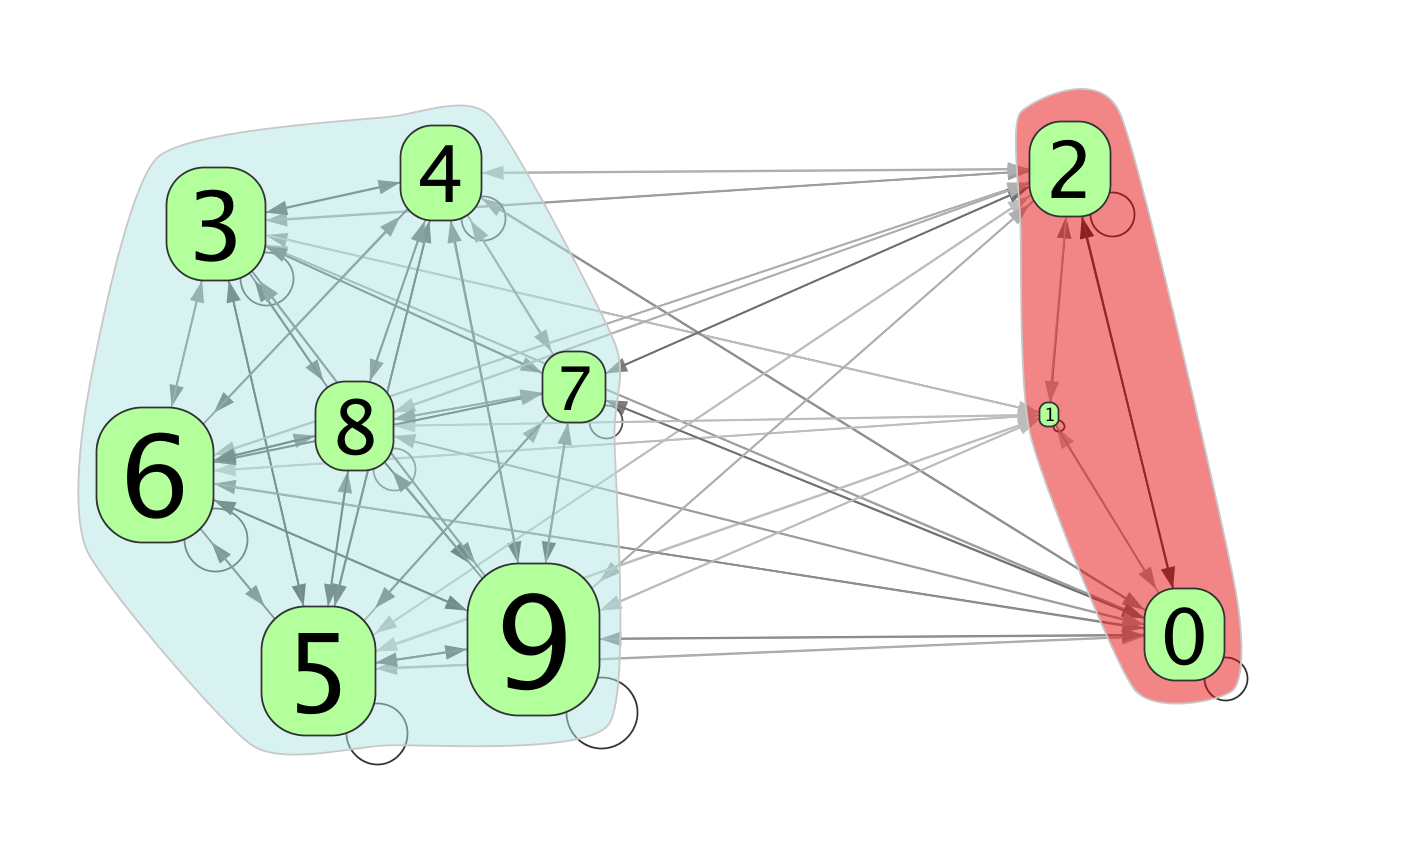
\includegraphics[scale=.3]{hier.png}
\caption{Hierarchical Model Visualization indicating the membership of the states in the 10 macrostate model in the (coarser grained) 2 macrostate model}
\end{figure}

\subparagraph*{A useful trick}
When an overlay is applied, a new data column is created in the backing node table called ``mapping'' that specifies the index of the aggregate to which the node at that row belongs. MSMExplorer uses a custom layout algorithm to group nodes within the same overlaid (aggregate) state together, but if this isn't quite doing the job, use this ``mapping'' field to separate aggregate groups. To do this, select ``mapping'' from the \emph{X Axis} drop-down and press \emph{Show Axis} (press \emph{Show Axis} again to hide the axis but keep the layout).  

\subsection*{9. TPT}
Transition Path Theory provides a method to identify paths of highest reactive flux between two sets of states. MSMExplorer contains an implementation of TPT coupled with a mechanism to automatically generate TPT diagrams. There are two mechanisms to run TPT in MSMExplorer. 

\subparagraph*{State to State} 
The first is simplest, but may only be used to run TPT between sets of cardinality one. Make sure you are viewing the model with 10 macrostates, and remove any overlay by moving the overlay slider to ``None.'' Now, click on node 0 to select this as the source node, and ctrl-click on node 9 to select it as the target node. A new window, TPTView, will appear, with an automatically generated diagram of the 3 highest reactive flux paths between node 0 and node 9.  Here, the default visual encodings are different than in GraphView; node size indicates reactive flux through that node and edge weight indicates reactive flux along that edge. Select \emph{Color Mode} to color nodes by their membership in the source set (red), sink set (blue), or neither (green). Now, in the text box at the lower right labeled ``Num Paths,'' enter 1 to see only the highest reactive flux path, and then enter 5 to see the 5 highest reactive flux paths.  Image export can be performed from the \emph{Save Image} button, and some basic facilities are provided to customize the appearance of this graph -- such as sliders to adjust ranges for node size and edge weight -- but these are not as extensive as are available via Vis Settings in GraphView. Section 10 discusses how to unite GraphView and TPTView to produce TPT diagrams with GraphView's visual controls. 

\subparagraph*{Set to Set} 
To run TPT between Sets of states, select \emph{TPT Selector} on the Control Dock. Enter the label of the node your wish to search in the box at the bottom labeled ``search,'' and add that node to the source or target set using the corresponding \emph{Source} and \emph{Target} buttons. You may also remove a node from a set by selecting its number in the box representing the set and pressing \emph{Remove}. Additionally, a node may be selected on the graph and then added to one of the sets using the \emph{Get Selected} button, which will load the label of that node into the search box. Go to the 25 macrostate hierarchy level. Select \emph{TPT Selector}. Add nodes 0 and 1 to the source set and node 24 to the target set. Press \emph{Run TPT} to run. Note that if a source or target node is not visible, it may be because no paths involving involving that node are present in the top reactive paths for the number of visible paths indcated in the \emph{Num Paths} box. Close the TPT view.

\subsection*{10. Putting it together: TPT and GraphView}
In our discussion of hierarchies, we mentioned that the node field ``mapping'' gets created when a hierarchy is visualized. Similarly, when TPT is run, a slough of fields are created that may be used to manipulate visual encodings. We will show how to take advantage of this to produce a custom TPT diagram visualization.

Go to the hierarchy level with 25 states and ensure no overlay is showing. Make sure labels are visible (if not, select the \emph{Label} radio button in the Node Renderer box. Click on node 6 and control-click on node 24 to run TPT between the two nodes. Now, change the number of visible top paths to 4 using the \emph{Num Paths} box in the bottom right of the TPTView window. Close TPTView. Now, click \emph{Vis Settings} to open the Vis Settings panel. Click the \emph{Only TPT Visible} button at the bottom of the panel to hide all members of the graph (nodes and edge) that were not visible in TPTView. Set the \emph{Node Size Field} menu to ``flux'' so that node size varies with reactive flux through the node; adjust the upper thumb to get a good range for node sizes. Set \emph{Node Color Field} to tptGroup to color nodes by their membership in the source/target sets, and change the \emph{Palette} for Node Color to ``Cool'' (one of a set of Preset palettes). Select the \emph{Shape} radio buton to represent nodes as circles. Now, go to the \emph{Edge} tab in the Vis Settings panel. Change the \emph{Edge Color Field} and \emph{Edge Weight Field} to flux to color and size edges by the amount of flux traveling along each edge. Pull the rightmost thumb of the \emph{Weight Range} slider a bit to the right to create a nice weight gradient. Note that if edge and arrowhead colors are out of sync, this can sometimes be helped by changing the \emph{Scale Type} for Edge Color, and then changing back to the desired Scale Type. 

Close Vis Settings. To get a nice curve on the edges, press \emph{Edge Type} on the Control Dock. Open the Force Panel and make adjustments until you have approximately your desired layout, then press \emph{Stop Layout} and pull nodes manually to form a graph of your desired form. At this point, you should have something similar to the diagram below. 

\begin{figure}[h]
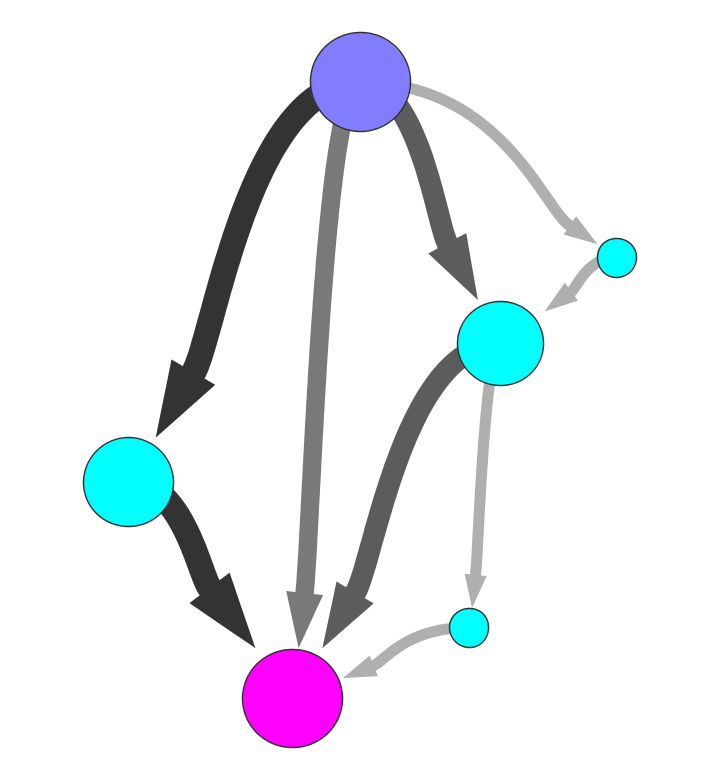
\includegraphics[scale=.3]{basicTPT.png}
\caption{Custom TPT Diagram without images}
\end{figure}

Now, we need to re-link with the images folder by going to \emph{File $\rightarrow$ Set Image Location} and selecting the folder \emph{demos/tutorial/images}. Now, press \emph{Show Images}. Open Vis Settings and go to the \emph{Label} tab; change the \emph{Rounding Radius} to 150 to make nodes round. Now tweak node layout by clicking and dragging nodes. When you have a result you are satisfied with, save by going to \emph{File $\rightarrow$ Save Image} and save the image as ``tptDemo.png''

\begin{figure}[h]
\includegraphics[scale=.3]{TPTdemo.png}
\end{figure}

\subsection*{Epilogue}

Congratulations, you have completed the MSMExplorer walkthrough! Make yourself a cup of coffee. 
\\

Questions and comments about this tutorial and anything MSMExplorer are welcomed at msmexplorer@gmail.com
\\

This document is released under the LGPL and the source is available at \texttt{http://github.com/brycecr/msmexplorer\_doc}
\\

MSMExplorer is also released under LGPL at 
\texttt{http://github.com/brycecr/msmexplorer}
\\

Please check out the README, REFERENCE$\_$TUTORIAL, and video(s) (at \texttt{http://vimeo.com/user13066911}) for more MSMExplorer learning resources. 
\\

\textbf{Happy MSMExploring!}

\end{document}
